\documentclass[12pt]{article}

\usepackage{sbc-template}
\usepackage{graphicx,url}
\usepackage[latin1,utf8]{inputenc}
\usepackage[brazil]{babel}
\usepackage[nonewpage]{imakeidx}
\usepackage[]{float} %Pacote que permite fazer posicionamento específico de figura com parâmetro [H]



\sloppy

\title{Modelagem de aplicativo para distribuição de informações}

\author{João Victor F. Consonni\inst{1}, Victor H. C. Leite\inst{1}, Matheus Ferreira\inst{1}, \\Matheus Milani\inst{1}, Artur L. Silva\inst{1}, Gustavo F. Fogolin\inst{1}, \\Bruno J. M. de Camargo\inst{1}, Danilo B. Cardoso\inst{1}, Daniel P. Cinalli\inst{1}, Lucas K. Kurokawa\inst{1}}

\address{Centro de Matemática, Cognição e Computação\\ Universidade Federal do ABC
  (UFABC)\\
  Av. dos Estados, 5001 - Bangú -- Santo André -- SP -- Brazil
  %\email{jconsonni, victor.costa, matheus.ferreira, milani.matheus, artur.lazarini, bruno.camargo, danilo.c@aluno.ufabc.edu.br}
  \email{\{jconsonni, victor.costa, matheus.ferreira, milani.matheus, }
  \email{artur.lazarini, gustavo.fogolin, bruno.camargo,}
  \email{danilo.c, dpcinalli, kenzo.kurokawa\}@aluno.ufabc.edu.br}
}
\begin{document} 

\maketitle

\begin{abstract} 
  Unified Modeling Language (UML) has become a standard in system modeling, from the requirements document to the maintenance phase of systems. Modeling allows customers and developers to view the system as a whole , understanding the connections between different classes and parts of the software. This document is intended to generate the diagrams requested by the client to assist in the implementation phase of the proposed mobile application.
\end{abstract}

\begin{resumo} 
   O unified Modeline Language (UML) se tornou um padrão na modelagem de sistemas, desde o documento de requisitos à fase de manutenção do sistemas. A modelagem permite que clientes e desenvolvedores possam visualizar o sistema como um todo de maneira mais completa, entendendo as conexões entre a  diferentes classes e partes integrantes do software. Este documento tem o intuito de gerar os diagramas requisitados pelo cliente, para auxiliarem na fase de implementação do aplicativo mobile proposto.
\end{resumo}

\newpage

\tableofcontents   

\newpage

\section{Introdução}
O principal foco de um software baseado em sistemas estruturados é de possibilitar aos desenvolvedores organizarem e visualizarem seus softwares de maneira ampla, fazendo uma abstração das necessidades de seu cliente, permitindo uma visualização do software como um todo antes mesmo do inicio de sua implementação. Esta visão possibilita o desenvolvimento de sistemas maiores e mais complexos, diminuindo custos e aumentando potencialmente evolução do sistema.\cite{chaudron2012effective}

O Unified Modeling Language (UML), ou linguagem unificada de modelagem em tradução livre, consiste de diferentes métodos de modelagem de sistemas amplamente utilizados por engenheiros de software, para organizar e estruturar os requisitos do sistema, a fim de gerar visualizações de um meta modelo do sistema funcional. Estes meta modelos por sua vez modelam mas  não mitigam todos os erros inerentes ao sistema que possam ocorrer durante a fase de implementação do software, entretanto reduzem muito a quantidade e seriedade de problemas que poderiam ocorrer sem uma modelagem adequada.\cite{Medvidovic:2002:MSA:504087.504088}

O documento de requisitos, gerado a partir de interações com o cliente final e a equipe de desenvolvimento, é o passo inicial para o inicio da modelagem do software. O documento de requisitos contem todos os aspectos funcionais, não funcionais e de domínio do software. Devido a sua linguagem simples, permite que o engenheiro de software entenda e apresente ao seu cliente e desenvolvedores de software, pontos guias para o entendimento do funcionamento do sistema. A partir dessa modelagem, os envolvidos no projeto podem observar as conexões entre requisitos, permitindo ao cliente uma ideia geral e aos desenvolvedores a lógica miníma para o desenvolvimento do código.

Os engenheiros de software que desenvolveram estes modelos necessitam periodicamente revisar e melhorar seus modelos, a fim de garantir que as necessidades do cliente estejam de acordo com o documento de requisitos, sempre focando em unificar, padronizar e reutilizar classes de elementos que possam ser evoluídos ou melhorados em outros projetos.

%\section{Diagrama de Classes}
%
%

\section{Diagramas de Estado}%Conteudo

Nesta seção serão apresentados os diagramas de estados que demonstram o funcionamento do aplicativo. Os diagramas foram modelados com base nos requisitos estabelecidos anteriormente, sendo explicitado para cada diagrama quais requisitos foram satisfeitos.

\subsection{Diagrama de Estados de Login}

O diagrama de estados a seguir mostra o processo de login por diversos métodos e cadastro de usuários, até a tela principal, de onde pode-se partir para o cadastro de incidentes e visualização de incidentes, que serão mostrados nas próximas seções. Dentre os requisitos estabelecidos, este diagrama implementa os seguintes: TI01, TI02, TI03, TI04, TI05, TI06 e CI02.

  \begin{figure}[!htb]
    \center{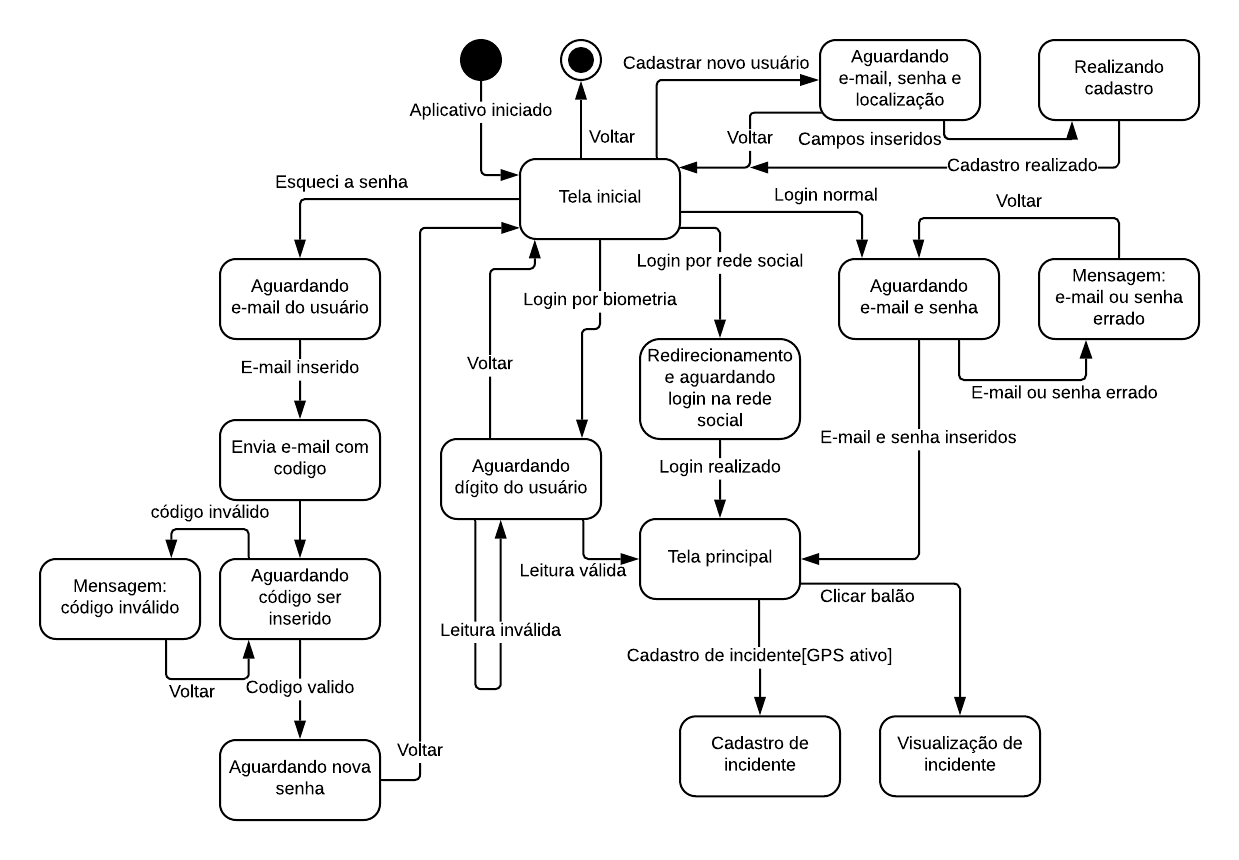
\includegraphics[width=\textwidth]
    {imagens/diagEstadoLogin}}
    \caption{\label{fig:diagEstadoLogin} Diagrama de Estados de Login}
  \end{figure}

\vfill%vfill para consertar pagebreak
\pagebreak%Quebra de página para consertar imagens

\subsection{Diagrama de Estados de Cadastro de Incidentes}

Neste diagrama de estados, é mostrado o processo de cadastro de um novo incidente por um usuário. Aqui pode-se visualizar o processo de inserção de dados e foros do incidente. Neste diagrama são satisfeitos os requisitos CI01, CI03, CI04, CI06, CI07, CI08, CI09.

  \begin{figure}[!htb]
    \center{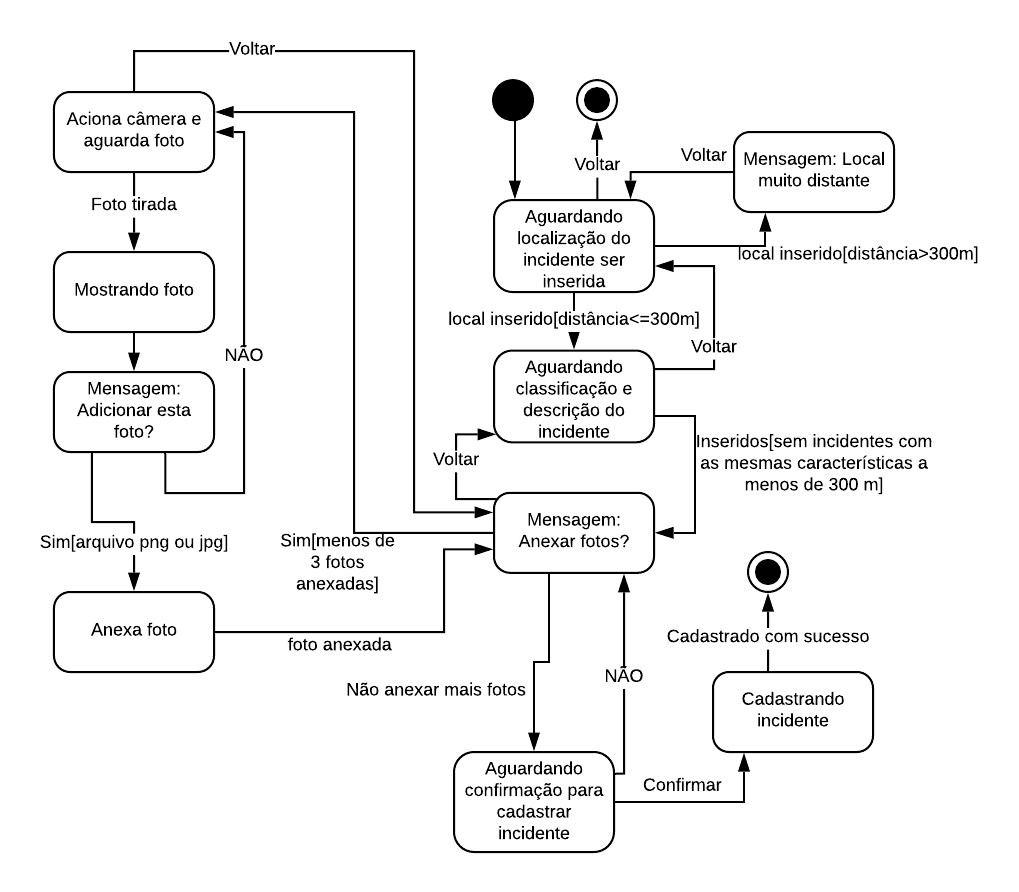
\includegraphics[width=\textwidth]
    {imagens/diagEstadoCadastroIncidente}}
    \caption{\label{fig:diagEstadoCadastroIncidente} Diagrama de Estados de Cadastro de Incidente}
  \end{figure}

\vfill%vfill para consertar pagebreak
\pagebreak%Quebra de página para consertar imagens

\subsection{Diagrama de Estados de Visualização}

No diagrama a seguir, é mostrado a visualização que um usuário terá ao clicar um balão de incidente no mapa. Quando o usuário for aquele que cadastrou o incidente sendo visualizado, terá a opção de editá-lo, como poderá ser visto no diagrama em \ref{fig:diagEstadoEdicao}. Os requisitos presentes neste diagrama são: VI01, VI02, VI03, VI04, VI05, VI06, VI07, VI08, VI09, VI10 e CI05.

  \begin{figure}[!htb]
    \center{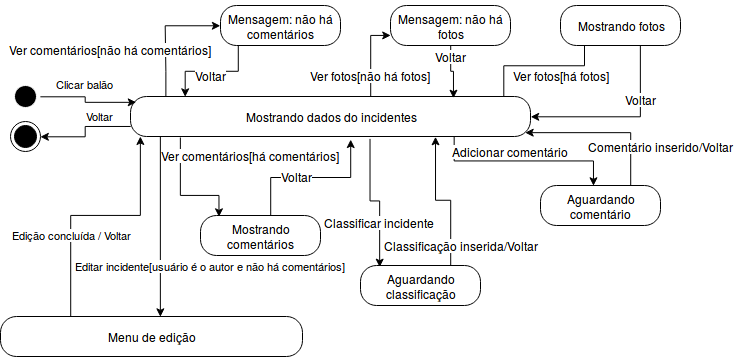
\includegraphics[width=\textwidth]
    {imagens/diagEstadoVisualizacao}}
    \caption{\label{fig:diagEstadoVisualizacao} Diagrama de Estados de Visualização}
  \end{figure}

\vfill%vfill para consertar pagebreak
\pagebreak%Quebra de página para consertar imagens

\subsection{Diagrama de Estados de Edição}
\label{subsec:diagEstadoEdicao}

Neste diagrama são apresentadas as opções de edição para um incidente, possibilitando alterar a descrição, classificação e fotos anexadas. os requisitos satisfeitos neste diagrama são: EI01, EI02 e EI03.

  \begin{figure}[!htb]
    \center{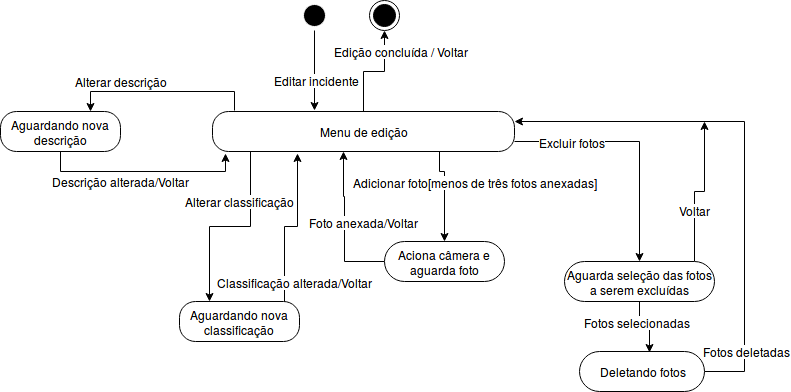
\includegraphics[width=\textwidth]
    {imagens/diagEstadoEdicao}}
    \caption{\label{fig:diagEstadoEdicao} Diagrama de Estados de Edição}
  \end{figure}

\vfill%vfill para consertar pagebreak
\pagebreak%Quebra de página para consertar imagens

\subsection{Diagrama de Estados de Incidente Passado}

Neste diagrama, é mostrado como um incidente será removido devido à sua classificação como Incidente Passado. Aqui são satisfeitos os requisitos CI10, RI01 e RI02.

  \begin{figure}[!htb]
    \center{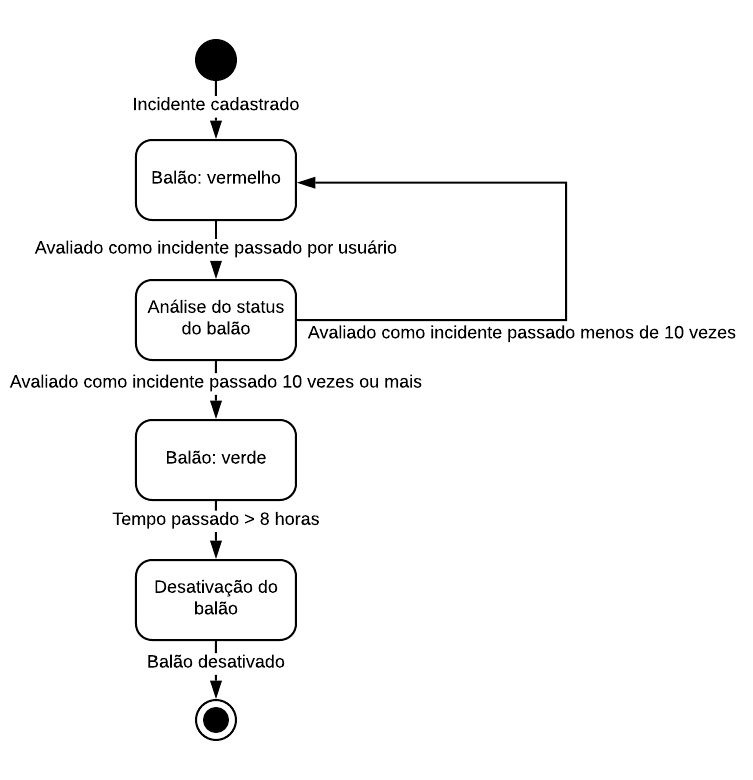
\includegraphics[width=\textwidth]
    {imagens/diagEstadoIncidentePassado}}
    \caption{\label{fig:diagEstadoIncidentePassado} Diagrama de Estados de Incidente Passado}
  \end{figure}


\section{Diagrama de Classes} 

O diagrama de classes foi criado a partir dos requisitos já listados anteriormente. Nele utilizamos como classes os principais atuantes encontrados nos requisitos RC01, RC03 - RC07, RC08, RC09, RC10, RC17 e RC18. Para identificar os atuantes, foi feito uma análise sintática dos requisitos, listando os substantivos e verbos, fazendo uma análise desses para identificar classes, atributos e métodos. Selecionamos os principais atributos e métodos de cada classe, sempre nos baseando como estrutura de variáveis e ações da classe, afim de determinar o objeto que gastaríamos de representar no diagrama, compartilhando informações com todas as outras classes. Por exemplo a classe "Usuario", com seu atributo privado "nomeUsuario", toda a vez que iniciada uma nova instância, altera o valor do atributo para cada novo Usuário criado. 

Após criada uma tabela com as possíveis classes e seus respectivos atributos e métodos, foi feito o diagrama interligando as classes. Uma grande dificuldade para a elaboração do diagrama foi definir quais eram as classes em si a partir dos requisitos, além de realizar a interconexão delas, quais atributos viriam de outras classes e quais métodos intervinham em quais classes.


  \begin{figure}[!htb]
    \center{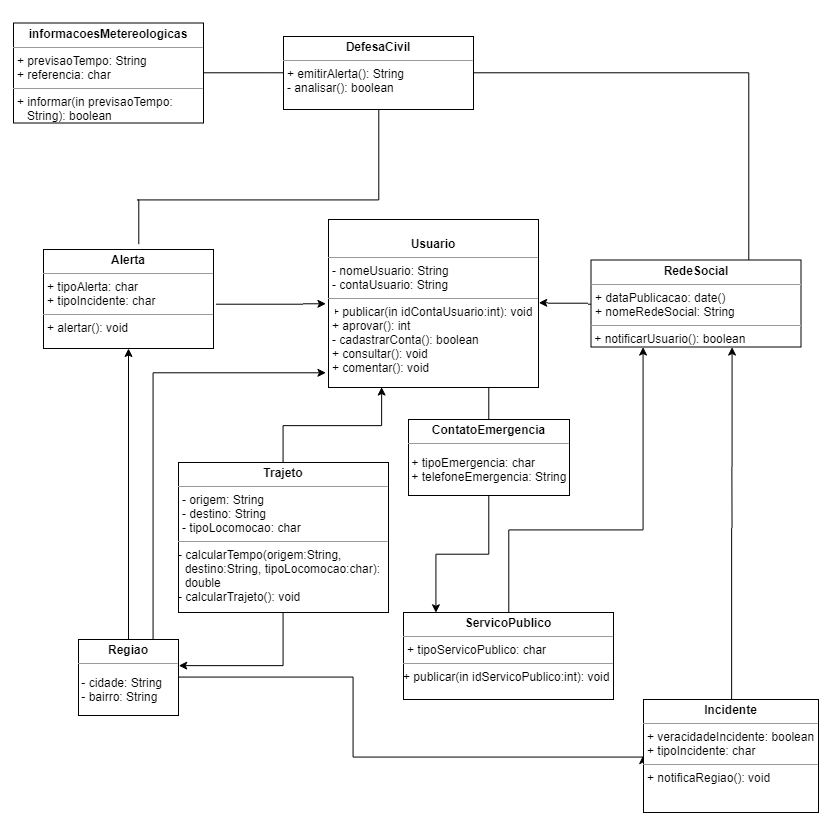
\includegraphics[width=\textwidth]
    {imagens/diagClasses}}
    \caption{\label{fig:diagClasses} Diagrama de Classes}
  \end{figure}

\vfill%vfill para consertar pagebreak
\pagebreak%Quebra de página para consertar imagens

\section{Diagramas de Atividade}%Conteudo

Nesta seção serão apresentados os diagramas de atividade, estes demonstram os fluxos de controle das atividades, dando ênfase ao fluxo de uma atividade para outra, tendo uma abordagem de alta abstração. Ele é um diagrama definido pela linguagem UML e representa os fluxos conduzidos por processamentos. Nesses diagramas podemos perceber como as atividades vão se comportar dentro do software em possíveis contexto e em conjunto com outras atividades.

Os diagramas foram desenvolvidos seguindo uma abordagem bem abstrata, tendo em vista que os diagramas de estado estão mais especificados. O intuito dos diagramas é tentando conectar e integrar os principais componentes (processos) do software, para demonstrar como eles funcionarão entre si. As principais dificuldades encontradas para o desenvolvimento foi conseguir entender o processo como sempre tendo início e fim, pois em alguns casos o processo parece cíclico, um outro ponto foi que a partir de alguns estados do diagrama poderíamos chegar a muitos outros, o que dificultou um pouco a modelagem pelo diagrama de atividades.

\subsection{Cadastro de Incidente}

Nesse diagrama é possível observar as etapas do cadastro de um novo incidente pelo usuário, onde uma parte do fluxo precisa estar completa para a validação e continuação do processo. Esse diagrama está relacionado com os seguintes requisitos: RC02, CI01, CI02, CI03, CI04, CI06, CI08, CI10.

  \begin{figure}[!htb]
    \center{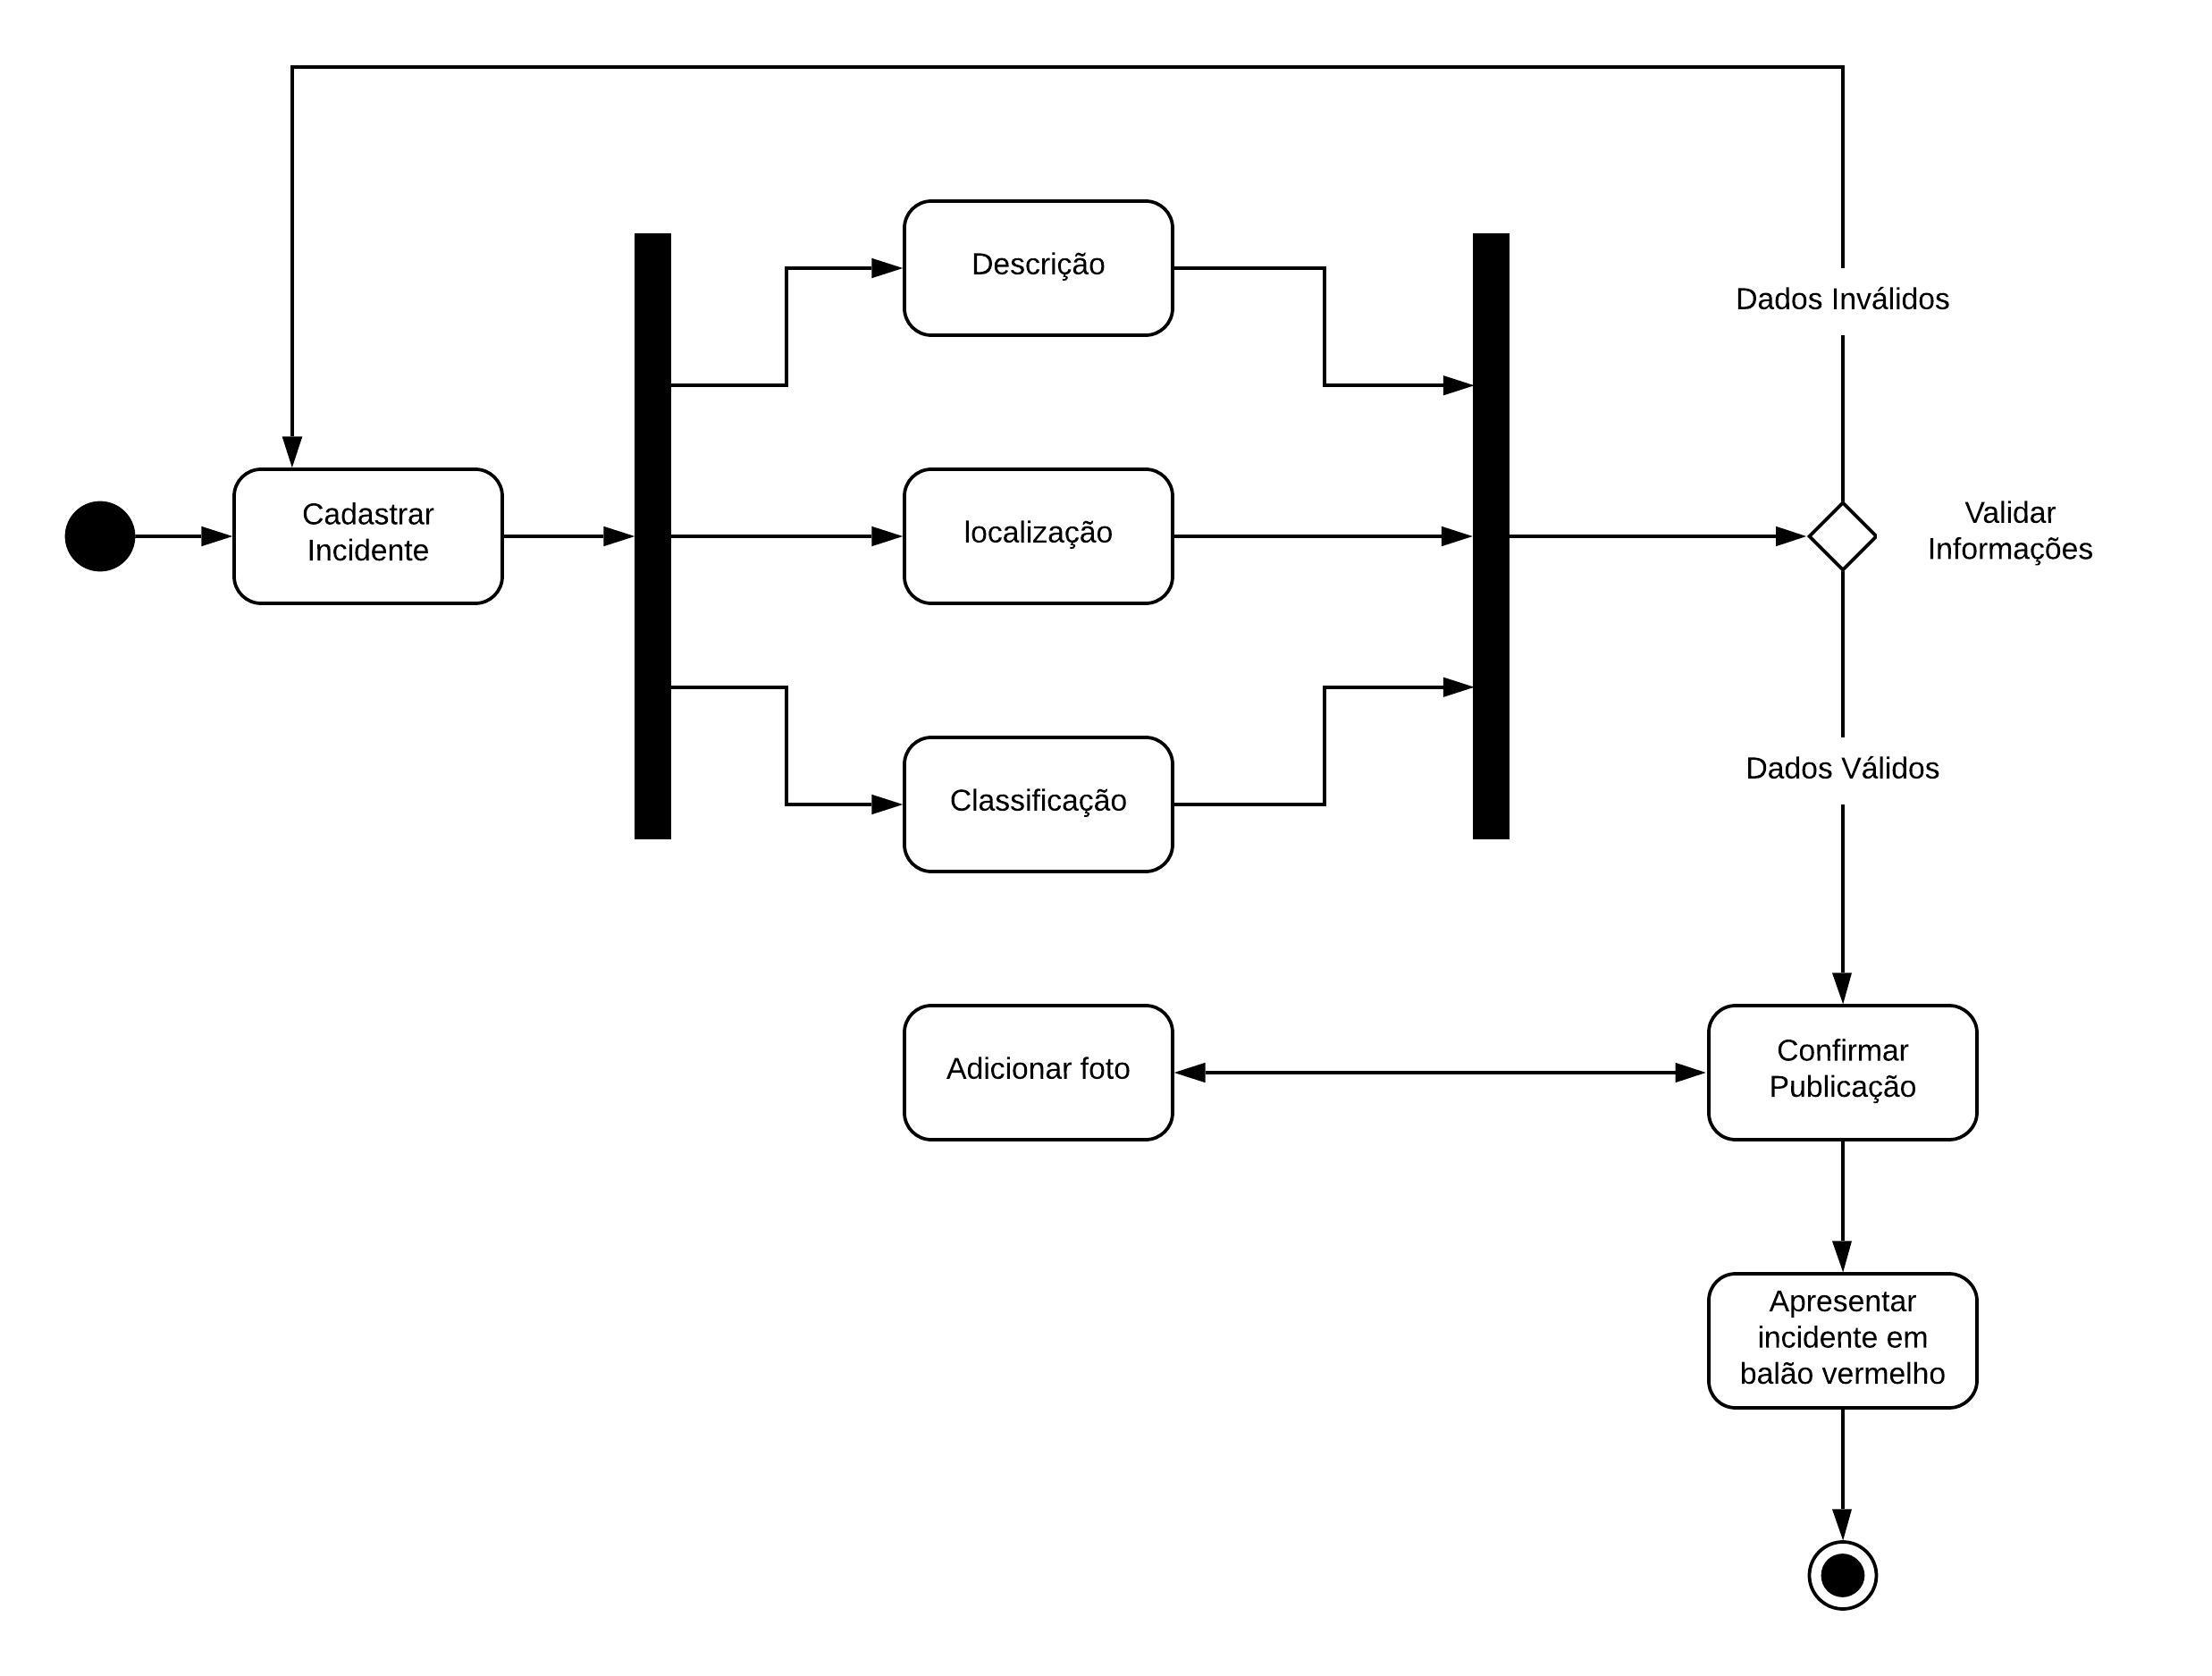
\includegraphics[width=\textwidth]
    {imagens/diagramasAtividades/atividadeCadastro}}
    \caption{\label{fig:diagCadastroInci} Diagrama de Atividade - Cadastro de Incidente}
  \end{figure}

\vfill%vfill para consertar pagebreak
\pagebreak%Quebra de página para consertar imagens

\subsection{Consulta de Incidente}

O diagrama a seguir demonstra como o usuário poderá consultar uma região do mapa, para verificar se há algum incidente nela através dos balões que deverão aparecer na tela caso exista. O diagrama está relacionado com os requisitos: RC09, TP01, TP06.

  \begin{figure}[!htb]
    \center{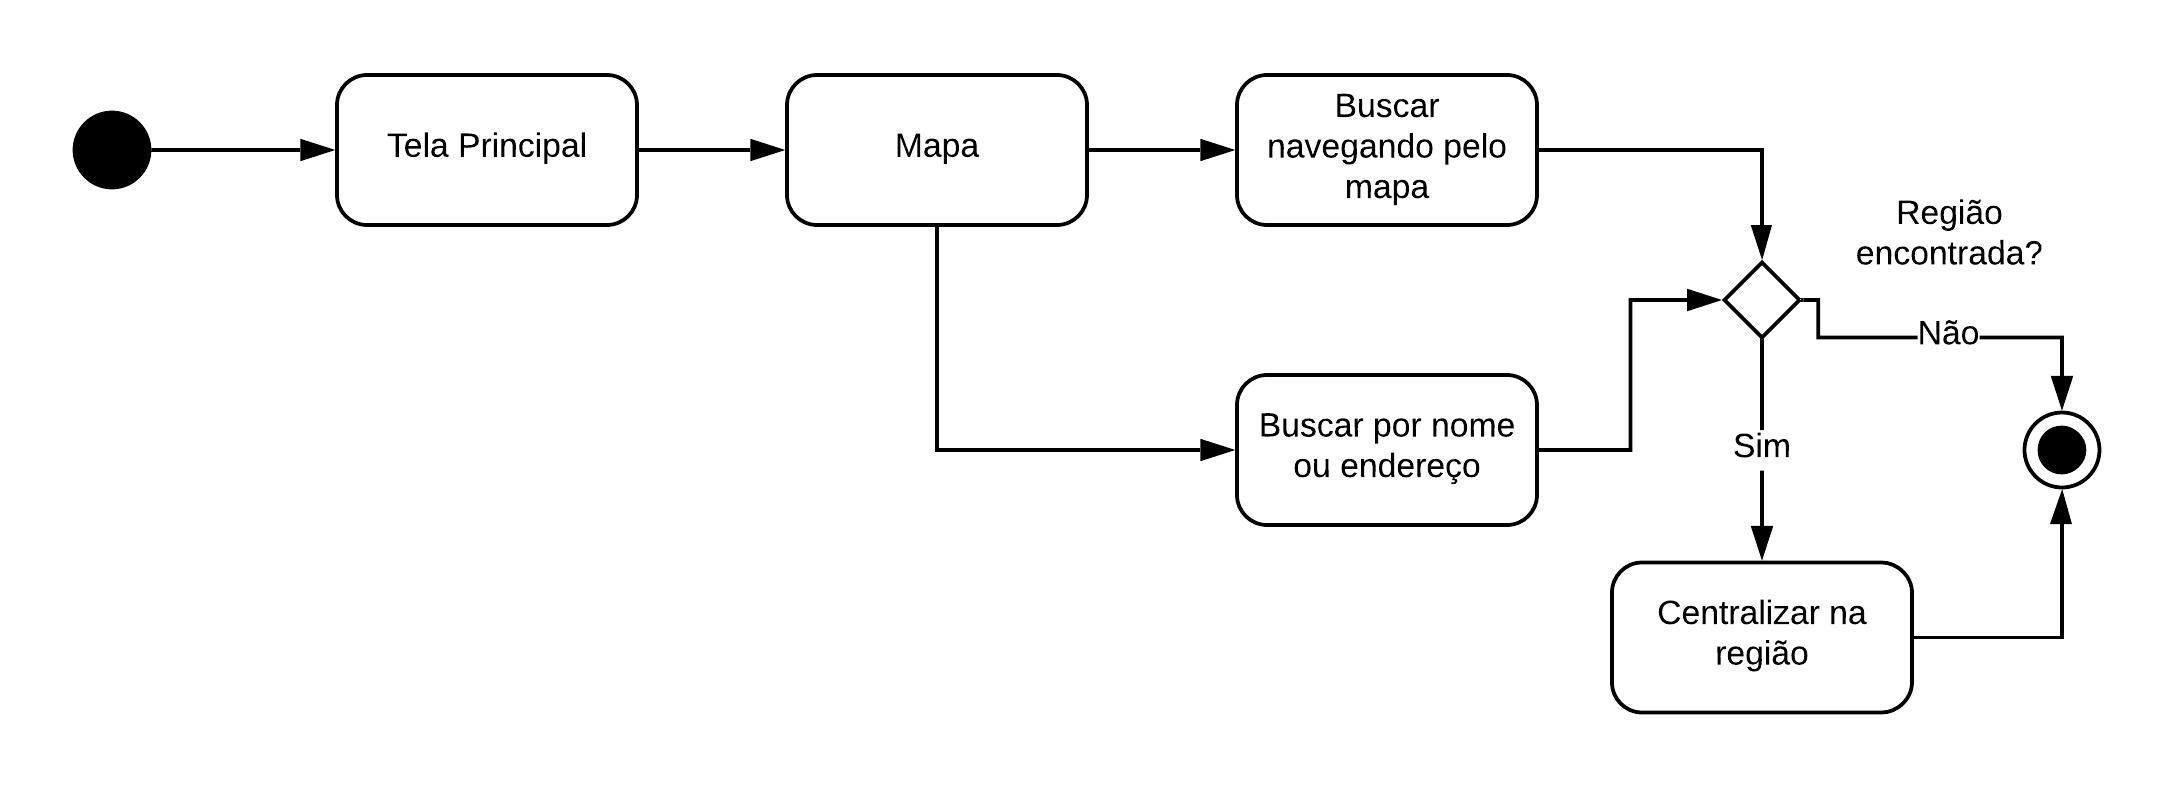
\includegraphics[width=\textwidth]
    {imagens/diagramasAtividades/atividadeConsulta}}
    \caption{\label{fig:diagConsultaInci} Diagrama de Atividade - Consulta de Incidente}
  \end{figure}

\vfill%vfill para consertar pagebreak
\pagebreak%Quebra de página para consertar imagens

\subsection{Login no Sistema}

O diagrama de login no sistema demonstra o processo que ocorre na primeira vez que o aplicativo é aberto em um dispositivo, ou após o logout. Nele temos as opções de login e de registro de uma nova conta. Requisitos relacionados: RC20, RC21, RC22, TI01, TI02, TI05, TI06.

  \begin{figure}[!htb]
    \center{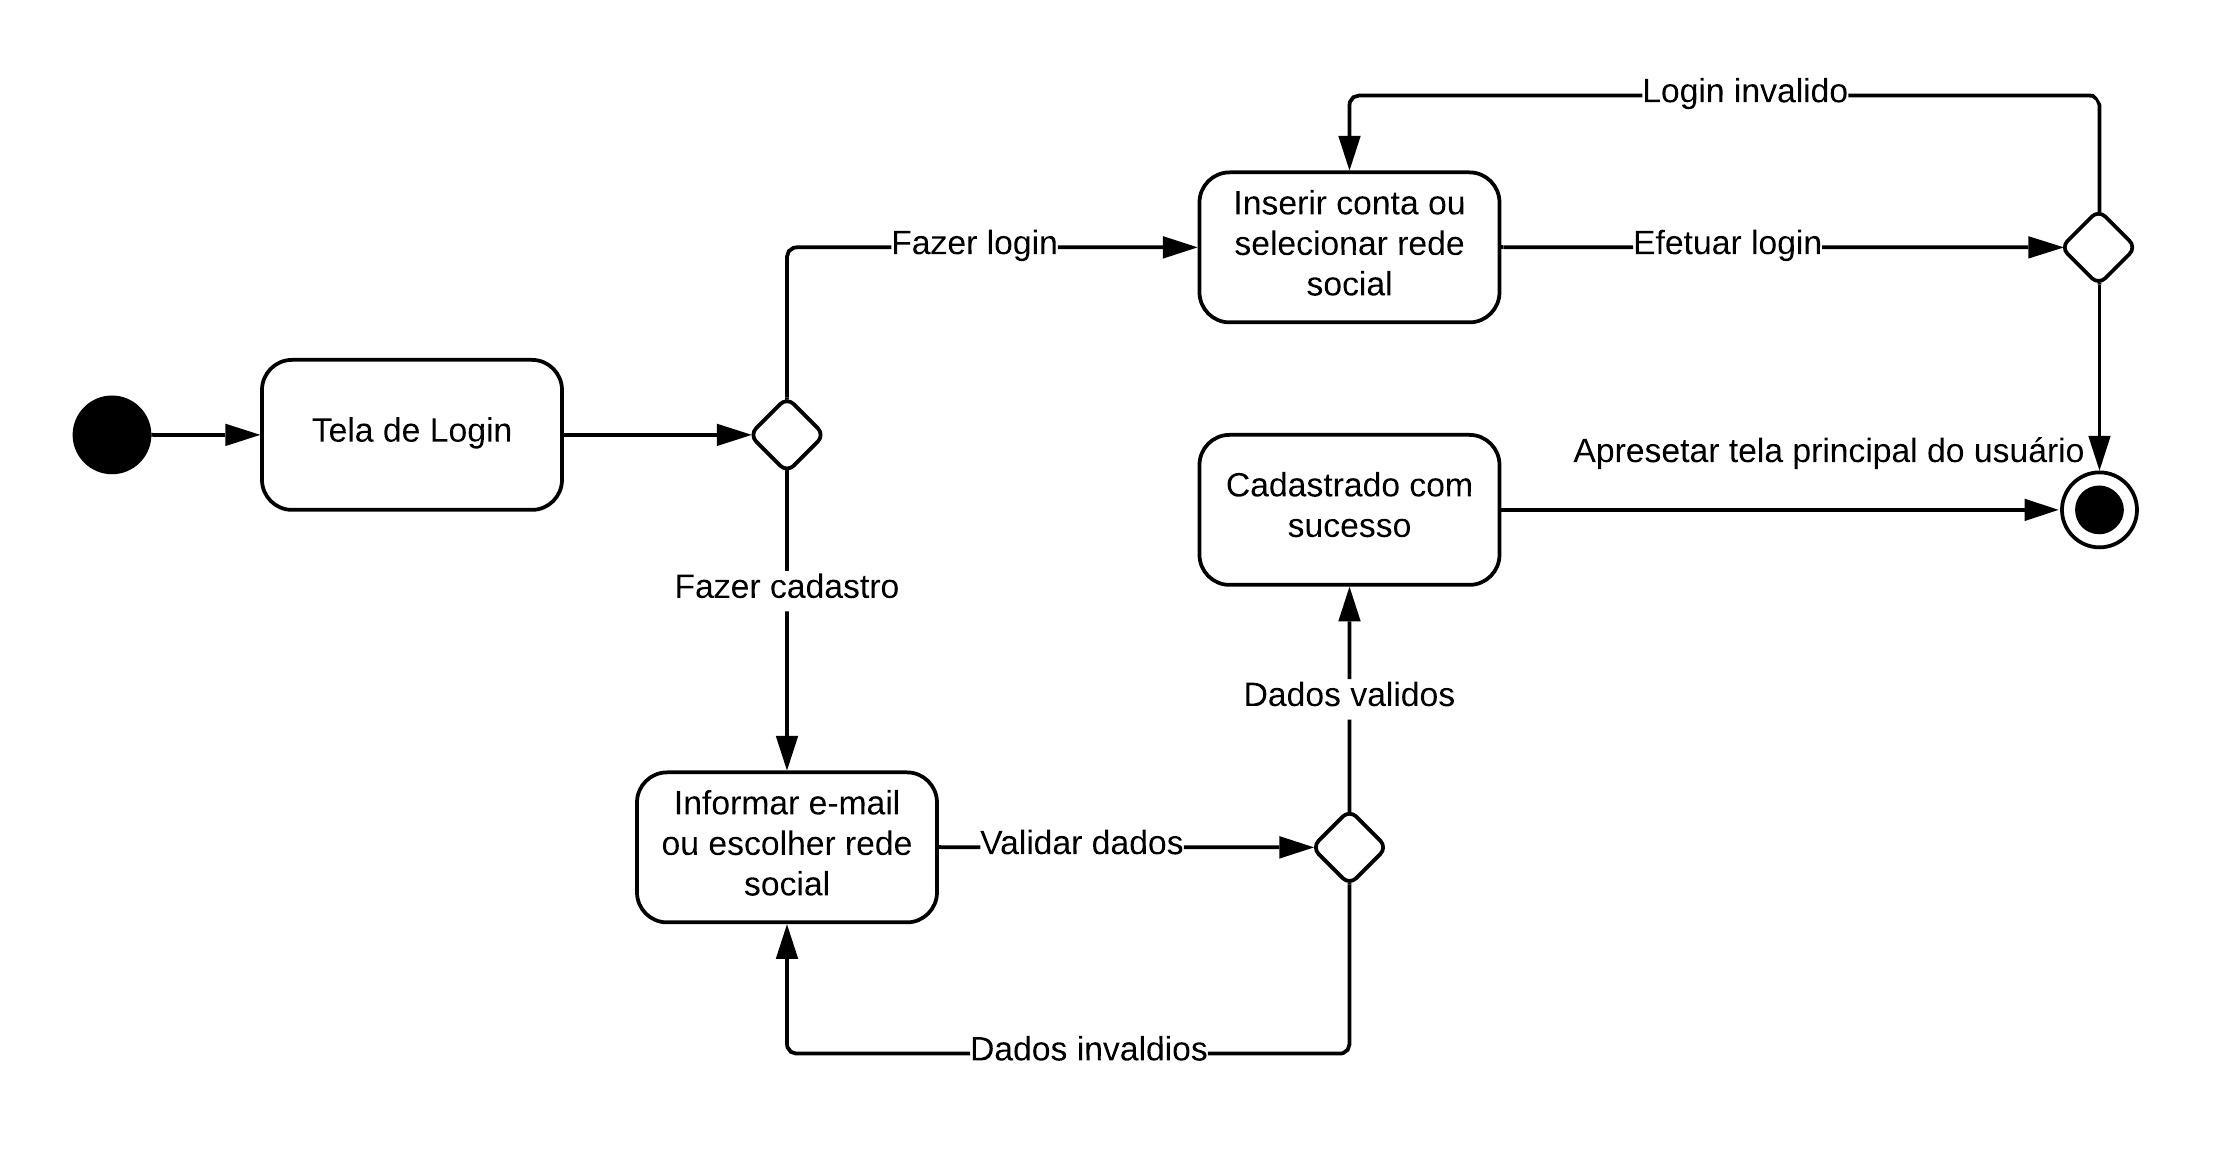
\includegraphics[width=\textwidth]
    {imagens/diagramasAtividades/atividadeLogin}}
    \caption{\label{fig:diagAtiviLogin} Diagrama de Atividade - Login no Sistema}
  \end{figure}

\vfill%vfill para consertar pagebreak
\pagebreak%Quebra de página para consertar imagens

\subsection{Tela Principal}

O diagrama de tela principal procura demonstrar as principais atividades que serão realizadas nessa tela, e no aplicativo. Dentre essas atividades temos a navegação no mapa e o cadastro e consulta de incidentes. O diagrama está relacionado com os requisitos: TP01, TP02, TP06, TP09, TP11, VI01.

  \begin{figure}[!htb]
    \center{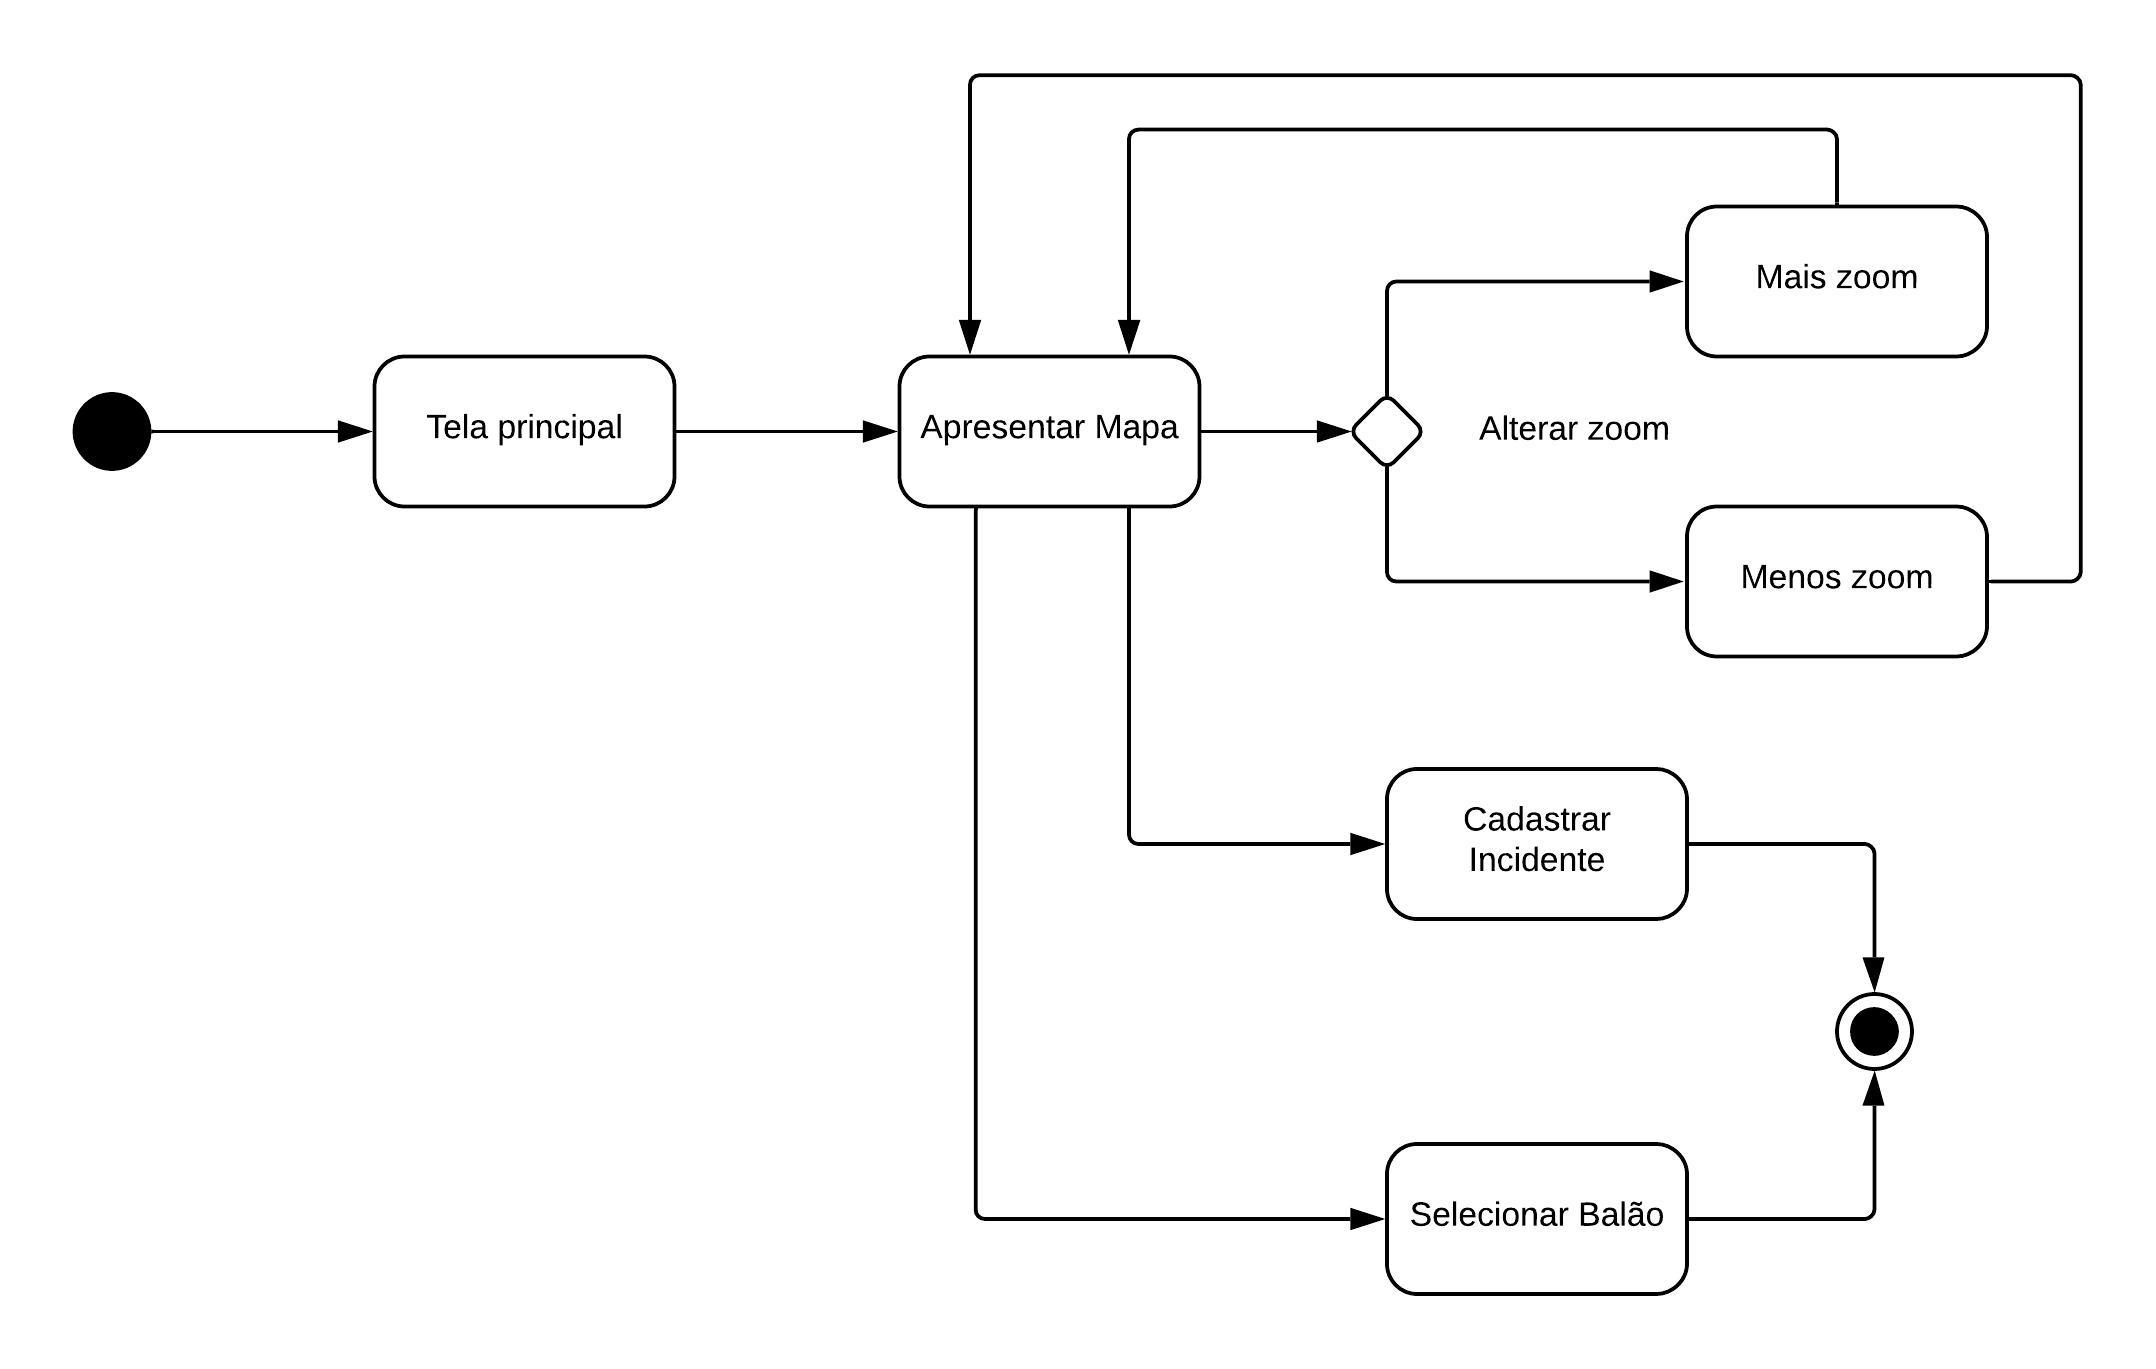
\includegraphics[width=\textwidth]
    {imagens/diagramasAtividades/atividadeTelaP}}
    \caption{\label{fig:diagTelaPr}nci Diagrama de Atividade - Tela Principal}
  \end{figure}

\vfill%vfill para consertar pagebreak
\pagebreak%Quebra de página para consertar imagens

\subsection{Visualização}

Esse diagrama demonstra como será feita a consulta de incidentes, onde o usuário deverá selecionar um balão no mapa para abrir a tela de visualização, nessa tela serão dispostas todas as informações do incidente. O disgrama representa como essas informações estarão dispostas. Relacionado com os requisitos: RC01, RC02, RC09, RC13, RC15, RC16, VI01, VI02, VI03, VI04, VI05, VI06, VI07, VI08, VI10.

  \begin{figure}[!htb]
    \center{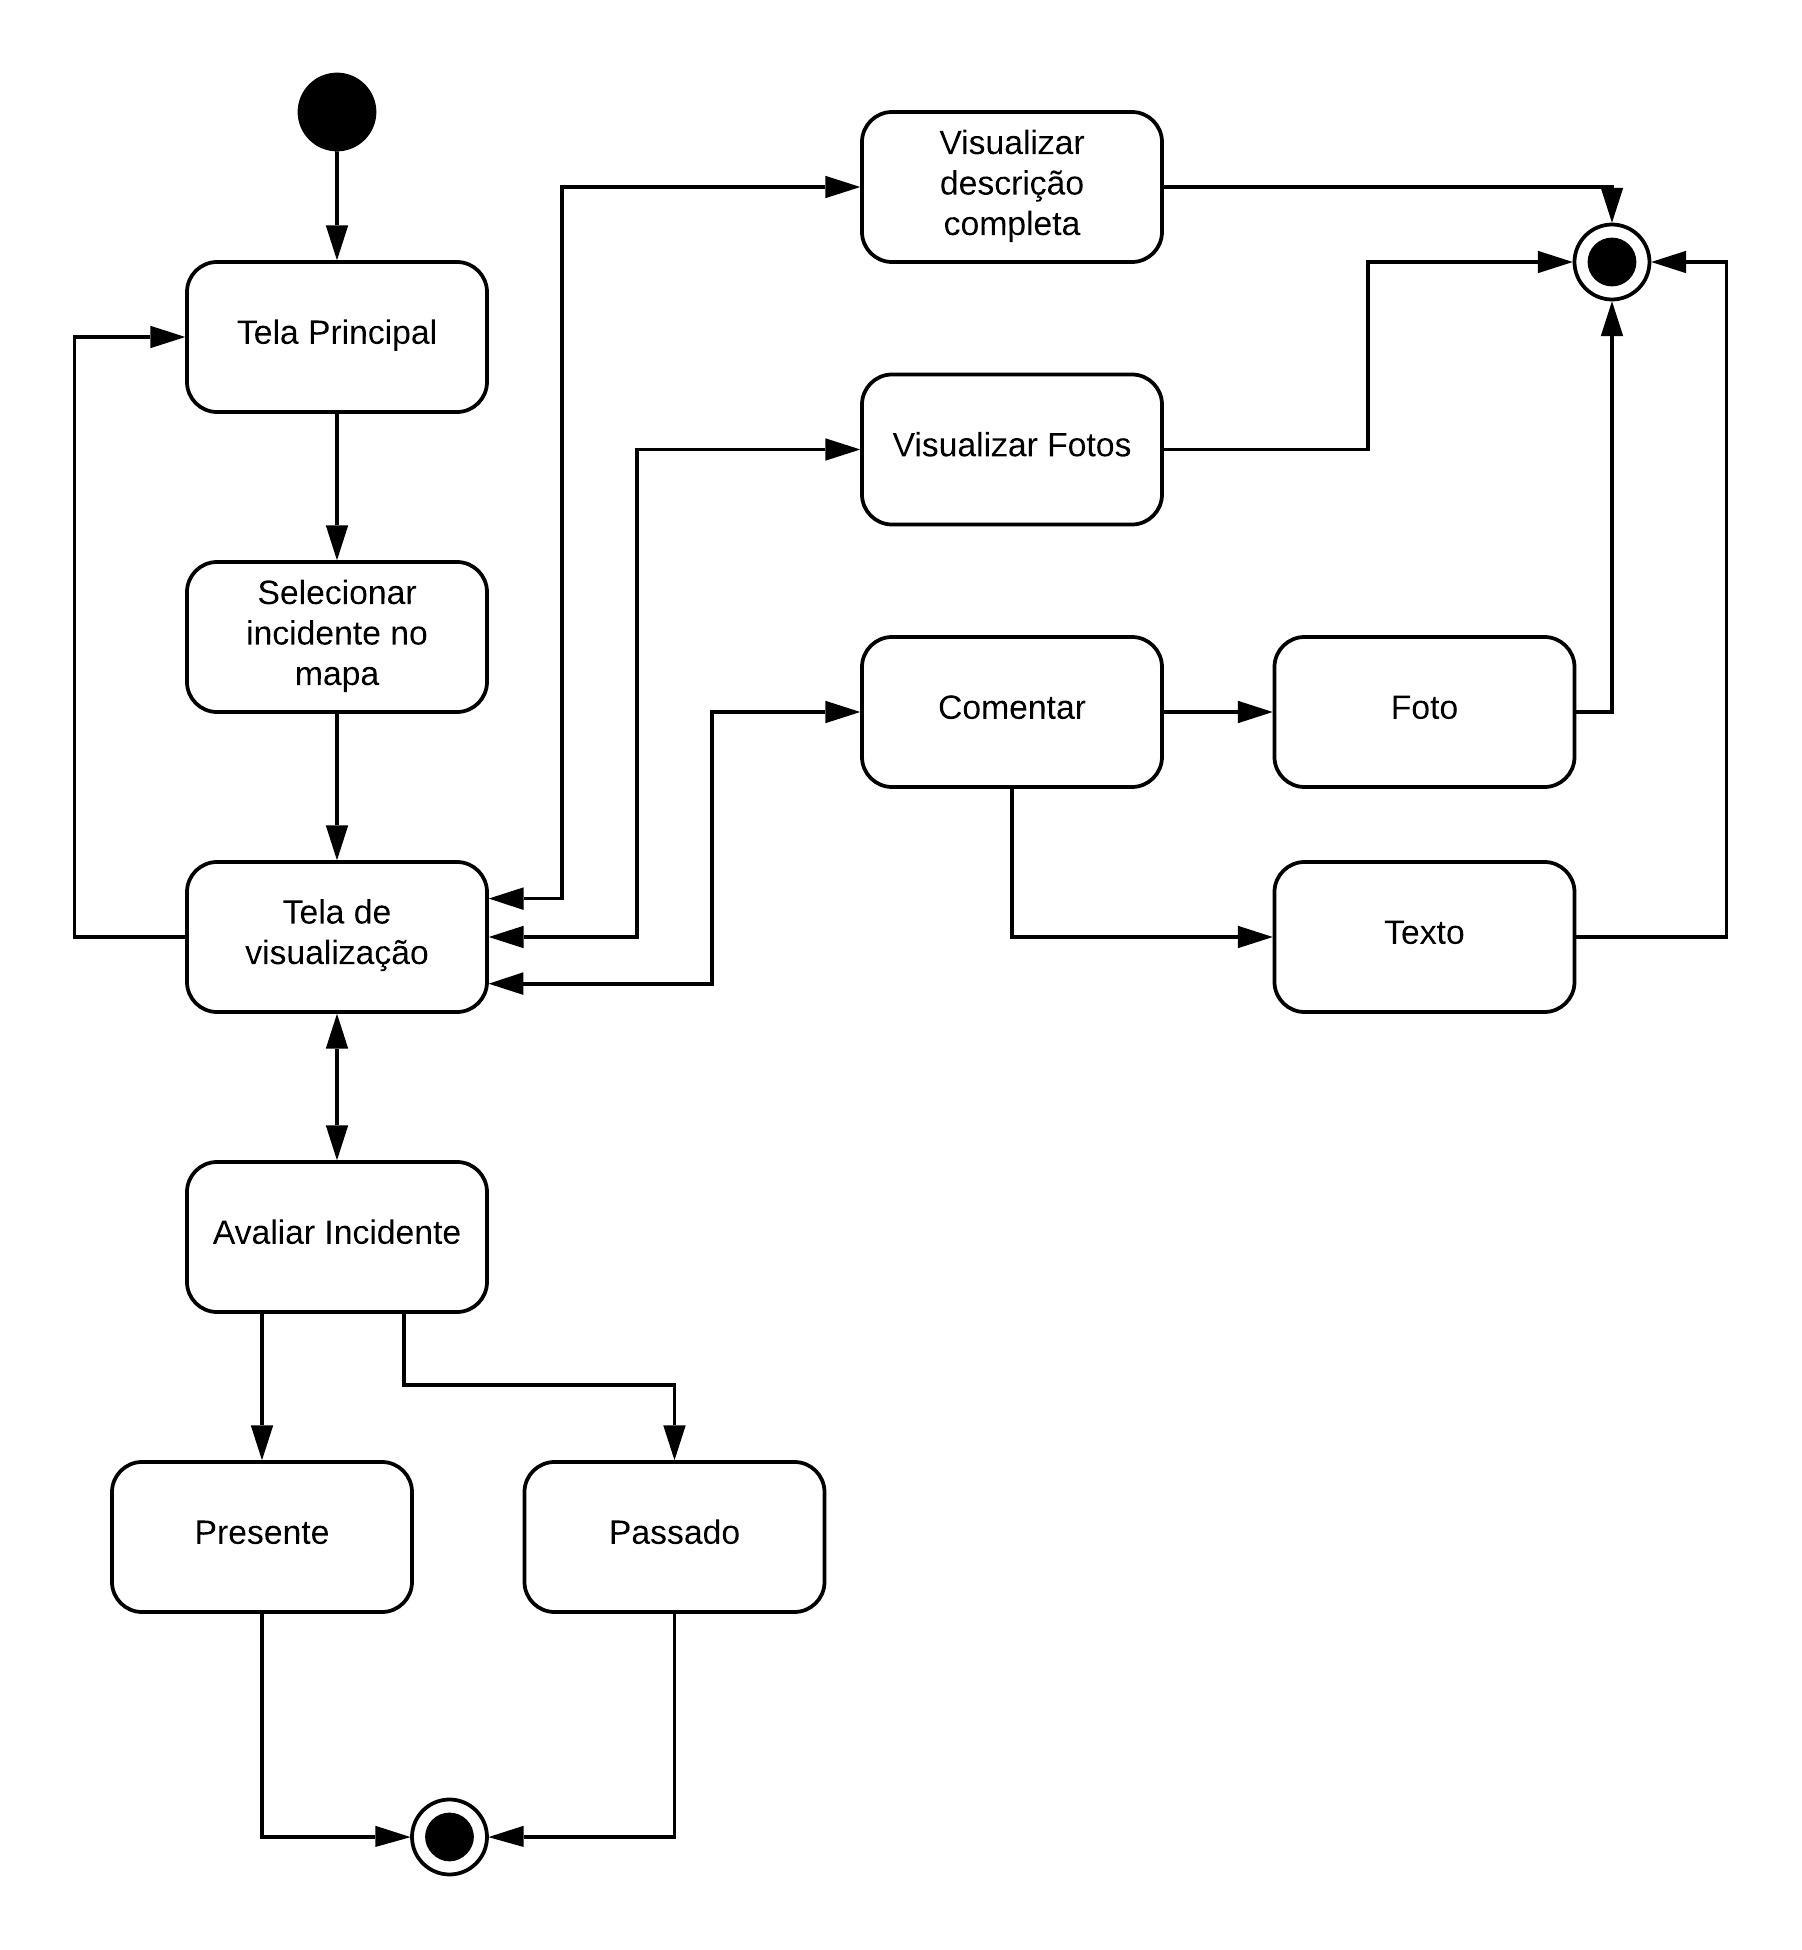
\includegraphics[width=\textwidth]
    {imagens/diagramasAtividades/atividadeVisu}}
    \caption{\label{fig:diagVisualizaInci} Diagrama de Atividade - Visualização}
  \end{figure}

\vfill%vfill para consertar pagebreak
\pagebreak%Quebra de página para consertar imagens

\section{Diagramas de Casos de Uso}

\subsection{Caso de uso: Login}
Este diagrama foi escolhido para ser feito pois nele podemos ver como é o processo de login deste sistema. Ele atende os requisitos de cliente: RC20, RC21, RC22, RC23, RC24, e os requisitos funcionais: TI01, TI02, TI03, TI04, TI05 e TI06.

  \begin{figure}[!htb]
    \center{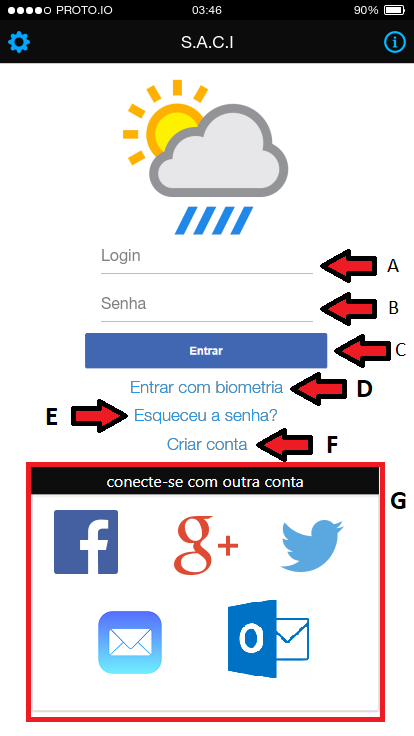
\includegraphics[width=0.6\textwidth]
    {imagens/diagramasCasosDeUso/login-DCU}}
    \caption{\label{fig:diagUseCase01} Diagrama de Caso de uso - Login}
  \end{figure}

\textbf{Ator principal}: Usuário

\textbf{Interessados e Interesses}:

\textbf{Usuário}: deseja acessar o sistema para consumir ou divulgar informações sobre a situação de uma determinada área.

\textbf{Pré condições}: o usuário está conectado a internet, possui conta cadastrada e está com aplicativo atualizado.

\textbf{Pós condições}: usuário consegue usufruir do sistema.

\textbf{Cenário de sucesso}:

1) Usuário coloca seu usuário (campo A).

2) Usuário coloca sua senha (campo B).

3) Aperta em entrar (botão C).

4) Usuário acessa o sistema e é redirecionado para próxima tela.

\textbf{Fluxos alternativos}:

Fluxo alternativo 1:

4) O sistema indica que o usuário não possui um cadastro válido, retorna à tela de login vazia.

Fluxo alternativo 2:

1) O usuário seleciona para acessar com biometria (Campo D). 

2) O aplicativo valida a biometria do usuário com a classe de segurança do sistema operacional do smartphone.

3) O sistema realiza o preenchimento e ações 1) à 4) do cenario de sucesso automaticamente.

Fluxo alterativo 3:

3) Caso a biometria do usuário não for cadastrada de acordo com o fluxo alternativo 2 ação 2), o aplicativo retorna a pagina de login vazia.

Fluxo alternativo 4:

1) Usuário coloca seu usuário (campo A).

2) Usuário clica em esqueceu a senha (Campo E).

3) Sistema envia ao e-mail cadastrado um link para alterar a senha do usuário.

Fluxo alternativo 5:

1) Usuário clica em "Criar conta" (Campo E).

2) Uma janela é apresentada, contendo campo de usuário (Campo A), campo de senha (Campo B) e campo para e-mail.

3) Aplicativo cadastra as informações no banco de dados.

Fluxo alternativo 6:

1) O usuário clica no ícone da rede social (em G) de preferencia para login automático.

2) O aplicativo redireciona ao site ou aplicação da rede social para login.

3) O servidor da rede social valida a informação inserida pelo usuário.

4) O servidor retorna ao aplicativo com as informações compartilhadas de login (Campo A) e senha (Campo B).

5) Aplicativo executa ação 4) do cenário de sucesso.

\vfill%vfill para consertar pagebreak
\pagebreak%Quebra de página para consertar imagens

\subsection{Caso de uso: ver mapa}
Este diagrama foi escolhido para ser feito pois nele podemos ver como será a experiência do cliente ao visualizar as publicações no mapa. Ele atende os requisitos de cliente: RC01 e RC09, e os requisitos funcionais: TP01, TP02, TP03, TP04, TP05, TP06, TP07, TP10 e TP11.

  \begin{figure}[!htb]
    \center{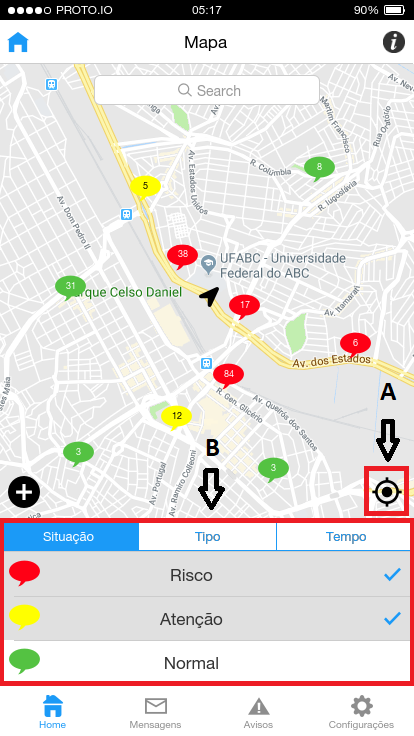
\includegraphics[width=0.6\textwidth]
    {imagens/diagramasCasosDeUso/Mapa-DCU}}
    \caption{\label{fig:diagUseCase02} Diagrama de Caso de uso - Ver Mapa}
  \end{figure}

\textbf{Ator principal}: usuário

\textbf{Interessados e Interesses}:

\textbf{Usuário}: deseja ver no mapa as publicações de seu local.

\textbf{Pré condições}: o usuário teve seu login autenticado e autorizou o compartilhamento de seu local.

\textbf{Pós condições}: usuário se informa sobre todas as publicações do local que está.

\textbf{Cenário de sucesso}:

1) Usuário aperta no ícone (em A) de localização em tempo real.

2) Escolhe (em B) os filtros para visualizar somente as informações que precisa.

3) Mapa é atualizado e só demostra as publicações de acordo com os filtros selecionados pelo usuário.

\textbf{Fluxos alternativos}:

Fluxo alternativo 1:

2) Aplicativo não tem permissão para saber localização do usuário

3) Usuário concede permissão

4) Continua em 2) do cenário de sucesso

Fluxo alternativo 2:

(1-3) Conexão do usuário cai, aplicativo para e fica aguardando restabelecer conexão.

\vfill%vfill para consertar pagebreak
\pagebreak%Quebra de página para consertar imagens

\subsection{Caso de uso: Notificação da defesa civil}
Este diagrama foi escolhido para ser feito pois nele podemos ver como será a experiência do cliente ao receber alertas da defesa civil, quando existir. Ele atende os requisitos de cliente: RC08, RC10, RC11 e RC12, e os requisitos funcionais: TP01, TP02, TP03, TP04, TP05, TP06, TP07, TP10 e TP11.

  \begin{figure}[!htb]
    \center{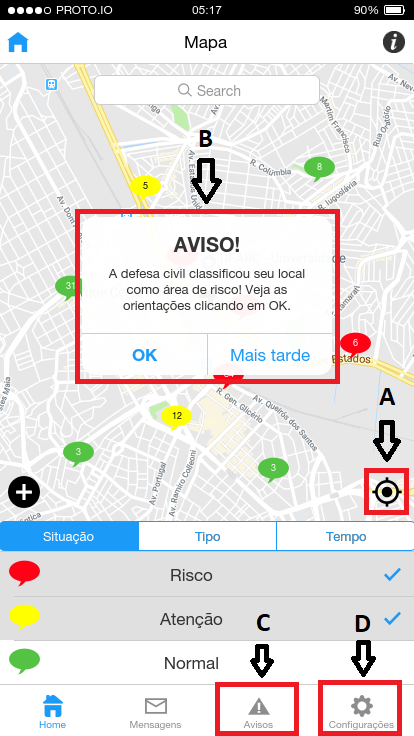
\includegraphics[width=0.6\textwidth]
    {imagens/diagramasCasosDeUso/DefCiv-DCU}}
    \caption{\label{fig:diagUseCase03} Diagrama de Caso de uso - Aviso da Defesa Civil}
  \end{figure}

\textbf{Ator principal}: Defesa Civil

\textbf{Interessados e Interesses}:

\textbf{1) Defesa Civil}: alertar os usuários do sistema em áreas de risco.

\textbf{2) Usuários}: receber alertas do sistema sobre as áreas de risco.

\textbf{Pré condições}: o usuário teve seu login autenticado, autorizou o compartilhamento de seu local em tempo real ou configurou regiões que gostaria de receber notificações.

\textbf{Pós condições}: usuário fica informado sobre as áreas de risco e, caso queira, receba orientações do que deve fazer.

\textbf{Cenário de sucesso}:

1) Usuário compartilha localização (em A). 

2) Por estar em uma zona de risco e existir um aviso da defesa civil, recebe uma notificação (em B).

3) Usuário aperta botão "OK" (em B) e recebe orientações sobre ações que deve tomar para sua segurança.


\textbf{Fluxos alternativos}:

Fluxo alternativo 1:

2) Aplicativo não tem permissão para saber localização do usuário

3) Usuário concede permissão

4) Continua em 2) do cenário de sucesso

Fluxo alternativo 2:

2) Não está em zona de risco. Encerra o fluxo.

Fluxo alternativo 3:

2) Está em zona de risco, mas não existe um aviso da defesa civil. Encerra fluxo.

Fluxo alternativo 4:

3) Usuário aperta botão "Mais tarde". Encerra fluxo.

Fluxo alternativo 5:

3) Usuário aperta botão "Mais tarde".

4) Usuário ve ou reve os avisos na aba "avisos" (em C). Volta para 3) do cenário de sucesso.

Fluxo alternativo 6:

1) Em uma área cadastrada (em D) pelo usuário, existe um aviso da defesa civil, recebe uma notificação (em B). Volta para 3) do cenário de sucesso.

\vfill%vfill para consertar pagebreak
\pagebreak%Quebra de página para consertar imagens

\subsection{Caso de uso: criar uma publicação}
Este diagrama foi escolhido para ser feito pois nele podemos ver como será a experiência do cliente ao criar uma nova publicação em uma área próxima a ele. Ele atende os requisitos de cliente: RC02 e RC14, e os requisitos funcionais: CI01, CI02, CI03, CI04, CI05, CI10.

  \begin{figure}[!htb]
    \center{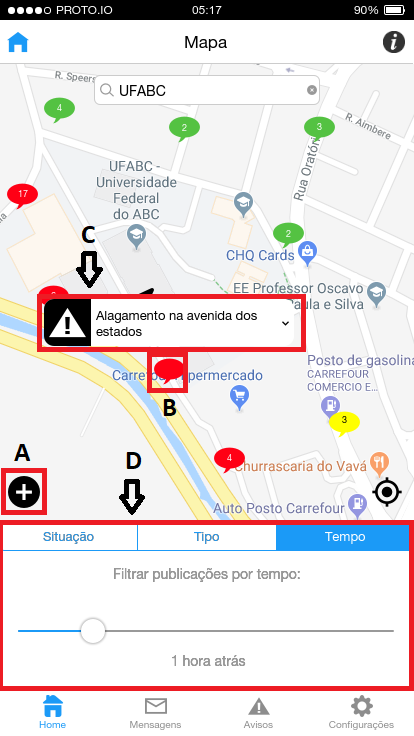
\includegraphics[width=0.6\textwidth]
    {imagens/diagramasCasosDeUso/Criar-DCU}}
    \caption{\label{fig:diagUseCase04} Diagrama de Caso de uso - Criar publicações}
  \end{figure}

\textbf{Ator principal}: Usuário

\textbf{Interessados e Interesses}:

\textbf{1) Usuários}: criar novas publicações em uma área ou local que ele está.

\textbf{Pré condições}: o usuário teve seu login autenticado, autorizou o compartilhamento de seu local em tempo real.

\textbf{Pós condições}: usuário divulga informações à outros usuários sobre novos incidentes.

\textbf{Cenário de sucesso}:

1) O usuário aperta o botão de cadastro (em A).

2) Seleciona o local do incidente dentro de sua área (em B).

3) Preenche o balão (em C) com um resumo breve.

4) Especifica (em D) características específicas sobre o incidente.

\textbf{Fluxos alternativos}:

Fluxo alternativo 1:

(1-4) Usuário desiste de criar uma publicação. Encerra o fluxo.

Fluxo alternativo 2:

(3-4) Usuário não preenche as informações obrigatórias. Encerra o fluxo.

\vfill%vfill para consertar pagebreak
\pagebreak%Quebra de página para consertar imagens

\subsection{Caso de uso: buscar uma publicação}
Este diagrama foi escolhido para ser feito pois nele podemos ver como será a experiência do cliente ao consultar alguma publicação de uma área que ele queira. Ele atende os requisitos de cliente: RC01 e RC09, e os requisitos funcionais: TP02, TP03, TP04, TP05, TP06, TP07, TP08, TP09, TP10 e TP11.

  \begin{figure}[!htb]
    \center{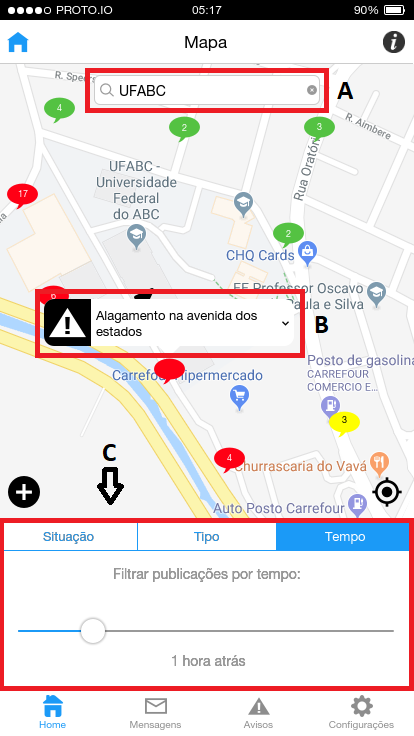
\includegraphics[width=0.6\textwidth]
    {imagens/diagramasCasosDeUso/Busca-DCU}}
    \caption{\label{fig:diagUseCase05} Diagrama de Caso de uso - Busca de publicações}
  \end{figure}

\textbf{Ator principal}: Usuário

\textbf{Interessados e Interesses}:

\textbf{1) Usuários}: listar publicações específicas em uma área ou local que ele tem interesse.

\textbf{Pré condições}: o usuário teve seu login autenticado.

\textbf{Pós condições}: usuário fica informado sobre as áreas de risco.

\textbf{Cenário de sucesso}:

1) O usuário faz busca (em A) de um local que deseja ver as publicações.

2) Ao selecionar alguma publicação, abre-se um balão (em B) contendo informações sobre a publicação.

3) Caso queira ver mais informações (comentários, imagens, etc) pode ser visto clicando na setinha na direita do balão (em B)


\textbf{Fluxos alternativos}:

Fluxo alternativo 1:

2) Insere local ou área inválida. Encerra fluxo.

Fluxo alternativo 2:

3) Não existem mais informações e o usuário não recebe nada.

Fluxo alternativo 3:

(1-3) Caso o usuário queira filtrar as publicações por tempo, tipo ou situação da publicação, pode ser feito (em C). Continua no cenário de sucesso em 2).

\vfill%vfill para consertar pagebreak
\pagebreak%Quebra de página para consertar imagens

\subsection{Caso de uso: Edição de publicação}
Este diagrama foi escolhido para ser feito pois nele podemos ver como será a experiência do cliente ao editar uma publicação de sua autoria. Ele atende os requisitos de cliente: RC15, RC16 e RC19 e os requisitos funcionais: EI01, EI03, VI01, VI03, VI08, VI09 e VI10.

  \begin{figure}[!htb]
    \center{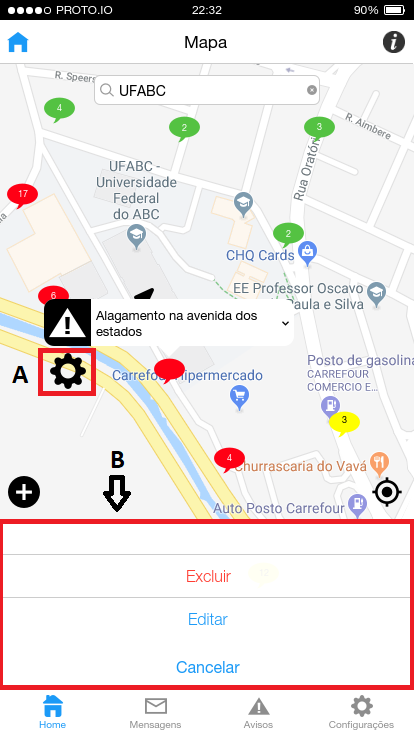
\includegraphics[width=0.6\textwidth]
    {imagens/diagramasCasosDeUso/edit-DCU}}
    \caption{\label{fig:diagUseCase06} Diagrama de Caso de uso - edição de publicação}
  \end{figure}

\textbf{Ator principal}: Usuário Autor da publicação

\textbf{Interessados e Interesses}:

\textbf{1) Usuários}: corrigir, deletar ou incrementar informações em uma publicação de autoria própria.

\textbf{Pré condições}: o usuário teve seu login autenticado e é o autor da publicação.

\textbf{Pós condições}: publicação está corrigida, incrementada ou excluída.

\textbf{Cenário de sucesso}:

1) Usuário clica no ícone de engrenagem (em A) de sua publicação.

2) Escolhe o que deseja fazer com sua publicação (em B).

3) Usuário decide editar a publicação.

4) Faz as alterações que deseja

5) Confirma.

6) Publicação é alterada.

\textbf{Fluxos alternativos}:

Fluxo alternativo 1:

(1-2) Usuário desiste de alterar publicação. Encerra o fluxo.

Fluxo alternativo 2:

3) Usuário decide excluir a publicação.

4) Confirma.

5) Publicação é excluída.

\vfill%vfill para consertar pagebreak
\pagebreak%Quebra de página para consertar imagens

\section{Diagramas de Sequência de Sistema}

\subsection{Descrição}
Para fazer esta seção, foram consultados os diagramas de casos de uso feitos e o documento de requisitos da segunda entrega. A partir desta consulta foram levantados os casos menos triviais a serem representados nos diagramas de sequência. Esta seção foi feita por Victor Hugo da Costa Leite e validada por João Consoni(PO). A principal dificuldade foi a de ver quais símbolos representariam melhor os pensamentos no diagrama de Remoção de Incidente.

\subsection{Fazer Login}
% Variável para controlar o tamanho de todos os DSS
\newcommand\dssDiagramWidth{0.8}
Abaixo encontra-se o diagrama de sequência de login. Nele o usuário acessa o aplicativo e insere o login e senha corretamente. Requisitos abordados: TI01.
  \begin{figure}[H]
    \center{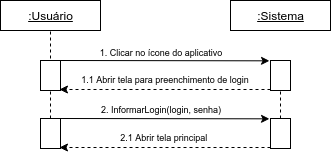
\includegraphics[width=\dssDiagramWidth\textwidth]
    {imagens/DSS//Login/dssLogin01.png}}
    \caption{\label{fig:dssLogin01} Diagrama de Sequência - Login e senha corretos pelo sistema.}
  \end{figure}
Abaixo encontra-se o diagrama de sequência de login. Nele o usuário acessa o aplicativo e insere o login ou senha errados. O sistema avisa que um dos dois está errado e o usuário tenta novamente até acertar login e senha. Requisitos abordados: TI01.
    \begin{figure}[H]
    \center{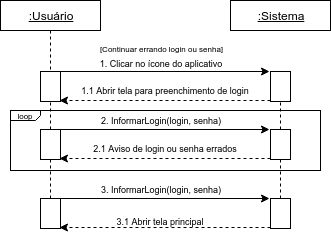
\includegraphics[width=\dssDiagramWidth\textwidth]
    {imagens/DSS//Login/dssLogin02.png}}
    \caption{\label{fig:dssLogin02} Diagrama de Sequência - Login e senha errados pelo sistema.}
  \end{figure}
No fluxo do diagrama abaixo o usuário escolhe acessar o sistema por meio de uma conta de rede social. Ao informar o login e a senha corretos o sistema consulta a rede social escolhida para validar os dados. Requisitos abordados: TI01 e TI02.
  \begin{figure}[H]
    \center{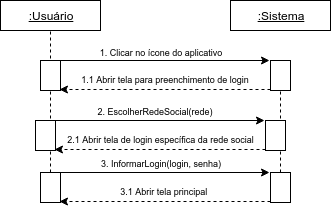
\includegraphics[width=\dssDiagramWidth\textwidth]
    {imagens/DSS//Login/dssLogin03.png}}
    \caption{\label{fig:dssLogin03} Diagrama de Sequência - Login e senha corretos por rede social.}
  \end{figure}
No fluxo do diagrama abaixo o usuário escolhe acessar o sistema por meio de uma conta de rede social. Ao informar o login ou a senha errados o sistema consulta a rede social escolhida para validar os dados. Tendo os dados não validados o sistema pede que o login e a senha sejam reinseridos novamente até que os dados corretos sejam validados. Requisitos abordados: TI01 e TI02.
  \begin{figure}[H]
    \center{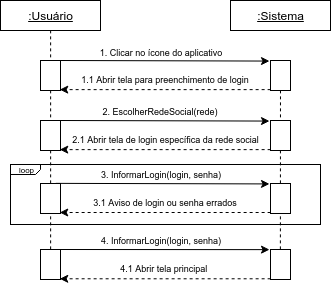
\includegraphics[width=\dssDiagramWidth\textwidth]
    {imagens/DSS//Login/dssLogin04.png}}
    \caption{\label{fig:dssLogin04} Diagrama de Sequência - Login e senha errados por rede social.}
  \end{figure}

\subsection{Notificação da defesa civil}
O diagrama de sequência abaixo representa o caso em que o usuário recebe uma notificação de que a defesa civil fez uma classificação para a área em que o usuário se encontra. Neste caso a notificação só é enviada para usuários presentes na região classificada. Requisitos abordados: RC10 e RNF16.
  \begin{figure}[H]
    \center{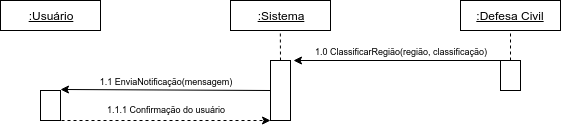
\includegraphics[width=1.0\textwidth]
    {imagens/DSS//Notificacao/dssNotificacao01.png}}
    \caption{\label{fig:dssNotify01} Diagrama de Sequência - Envio de notificação da defesa civil.}
  \end{figure}
\subsection{Inclusão de Incidente}

O diagrama abaixo representa o fluxo para que um incidente seja publicado. O usuário clica no botão criar publicação e informa os dados da publicação na ela que se abre. Ao final basta terminar a publicação. Requisitos abordados: CI01, CI04 e CI06.

  \begin{figure}[H]
    \center{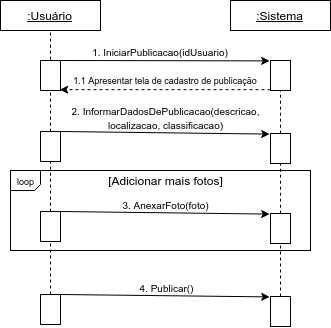
\includegraphics[width=\dssDiagramWidth\textwidth]
    {imagens/DSS//InclusaoPublicacao/dssPublicacao01.png}}
    \caption{\label{fig:dssPublic01} Diagrama de Sequência - Cadastro de novo Incidente.}
  \end{figure}

\subsection{Remoção de Incidente}

O diagrama abaixo representa o fluxo necessário para que uma publicação seja removida. Durante a consulta de uma publicação os usuários podem classificar a publicação como do tipo tempo passado. Caso isso seja feito o sistema verifica quantas classificações do tipo foram feitas. Se menos do que 10 classificações desse tipo foram feitas o sistema simplesmente incrementa o contador, caso contrário o sistema muda a representação do incidente de um balão vermelho para verde. 8 horas depois do balão estar na cor verde o balão deixa de ser mostrado no mapa da tela principal dos usuários. Requisitos abordados: VI10, RI01 e RI02.

\begin{figure}[H]
    \center{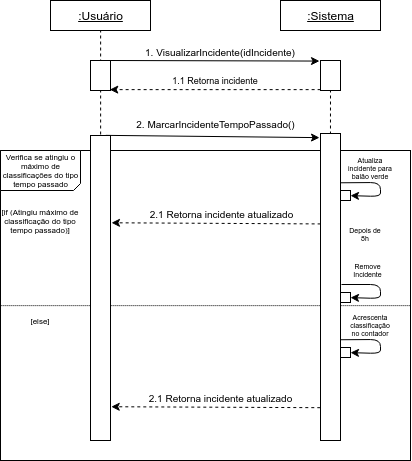
\includegraphics[width=1.0\textwidth]
    {imagens/DSS/RemocaoPublicacao/dssRemocao01.png}}
    \caption{\label{fig:dssRemo0e1v} Diagrama de Sequência - Remoção de Incidente.}
  \end{figure}

\section{Discussão}

Esta fase de projeto teve como objetivo externar e refinar o documento de requisitos, entregue na fase anterior. Assim como servir como base da documentação de desenvolvimento do software. 

Durante este processo pode ser percebido a importância de que cada modelo reflita os requisitos definidos na documentação anterior como norma. Pela introdução dos requisitos satisfeitos em cada diagrama houve como reflexo uma visão coerente do software que será construído que facilitará a introdução de melhorias nas documentações anteriores, como nas futuras, além da facilitação no processo de comunicação do projeto. 

Para as próximas fases de projeto este documento, assim como o documento de requisitos, terão grande importância tanto na comunicação com o cliente, por trazer diagramas como o de caso de uso, que facilitam a comunicação sobre as funcionalidades, além de trazer diagramas essenciais para equipe de desenvolvimento, como o diagrama de classes.  

\section{Conclusão}
O processo de modelagem de software tem um papel de extrema importância na qualidade geral do software ao término do desenvolvimento. A partir do documento de requisitos, documento que mapeia as funcionalidades do software baseado em frequentes conversas com o cliente em um processo de maturação da ideia que o cliente tem sobre o que ele espera do produto final, faz-se necessário uma análise mais aprofundada dos fluxos que estes requisitos levantados representam.

Com a interpretação dos requisitos, no contexto de como aplicação irá funcionar e como o usuário irá interagir com o software, obtêm-se uma visão melhor de como a aplicação deve ser estruturada para abranger todas as funcionalidades levantadas e, para a documentação desse processo de modelagem surgem diversos diagramas, que armazenam e auxiliam na transmissão dessas informações ao desenvolvedor, de forma clara e intuitiva.

O processo de criação desses diagramas e o processo de modelagem em si, no contexto deste projeto, foi bastante interessante pois fez com que revisitássemos os requisitos levantados anteriormente e discutíssemos melhor como seriam os relacionamento entre classes do sistema, de que forma o usuário iria interagir com a aplicação e ajudou na visualização dos fluxos principais. Este é de grande valor no processo de desenvolvimento, pois assim são tratados algumas ambiguidades que eventualmente não são percebidas durante o processo de levantamento dos requisitos e que impactariam negativamente na eficiência do processo de desenvolvimento.

\section{Informações de Apoio}
\subsection{Apêndices}
\subsubsection{Apêndice A - Descrever como o processo de Scrum foi seguido pela equipe}
Devido a grande evolução no projeto, a equipe vem assimilando bem o propósito e o modelo de trabalho ágil do Scrum. A dinâmica das entregas esta ficando mais fluída, a medida que nos acostumamos mais com os prazos de entrega e o esforço necessário para a Sprint.

Houve uma grande melhora na divisão das tarefas, muito devido a cerimonia de Planejamento (Planning) que foi realizada com maior qualidade comparada as anteriores. Aproveitamos mais o tempo pratico em sala e de la saímos com as principais tarefas da Sprint consolidadas para cada membro, o que agilizou os entregáveis.

Chegamos ao final de mais um Sprint e a evolução é nítida na equipe, a transparência e comunicação se faz presente em todos, importantíssimo para um método ágil de trabalho. Resta para agora nos adaptarmos a mudança de integrantes da equipe, bem como na liderança.
\bibliographystyle{sbc}
\bibliography{entrega_03_01}
\end{document}